\begin{frame}{Fronteiras}
    \begin{itemize} \setlength\itemsep{1em}
        \item Porém as fronteiras esntre biomas distíntos precisam ser suavizadas.
    \end{itemize}
    
    \begin{figure}[H]
        \centering
        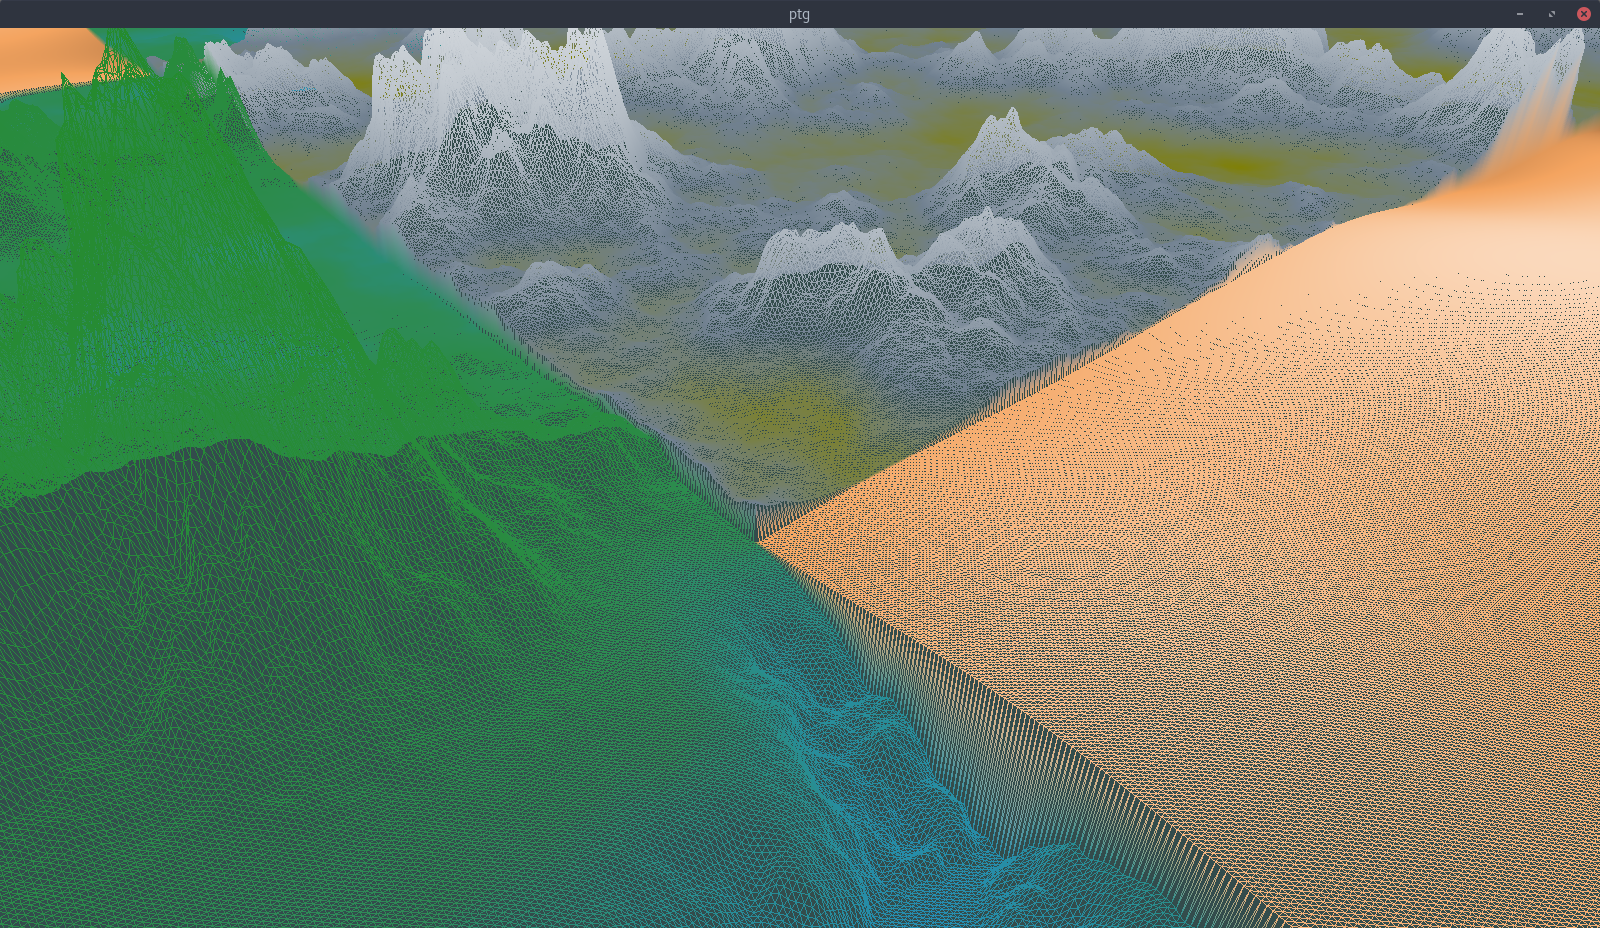
\includegraphics[width=.9\textwidth]{img/descontinuos.png}
        \caption{Fronteira entre biomas com descontinuidade.}
        \label{fig:descontinuos}
    \end{figure}
    
\end{frame}

\begin{frame}{Fronteiras}
    \begin{itemize} \setlength\itemsep{1em}
        \item Resolvendo o problema com interpolação.
    \end{itemize}
    
    \begin{figure}[H]
        \centering
        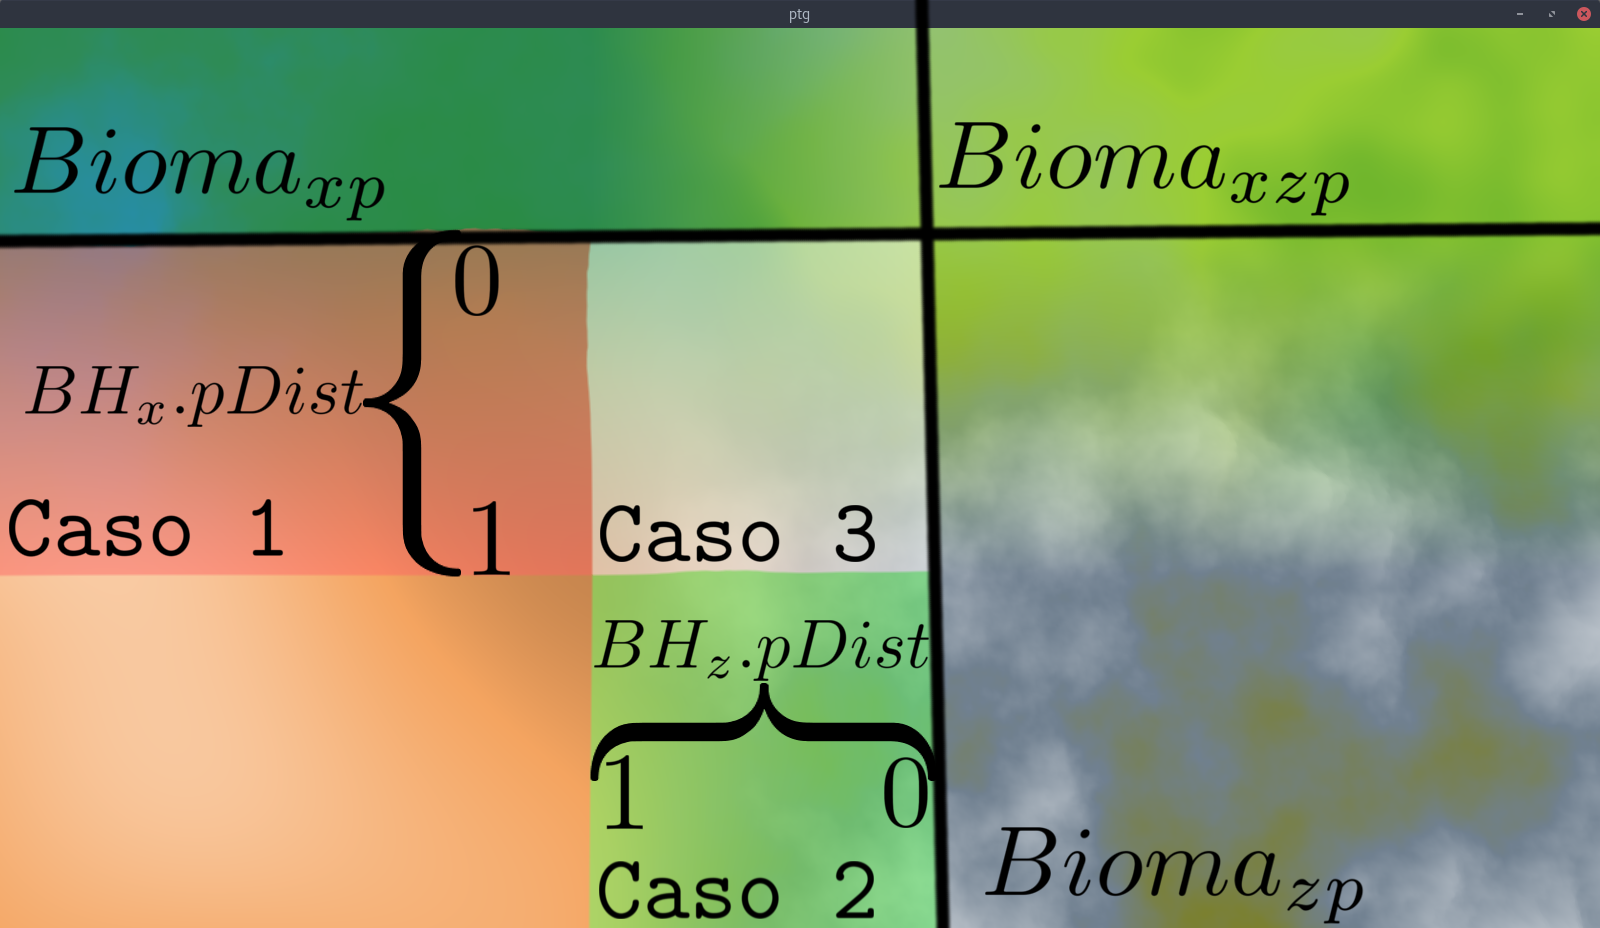
\includegraphics[width=.9\textwidth]{img/border/yeah.png}
        \caption{Fronteira entre biomas com descontinuidade.}
        \label{fig:img_border_yeah}
    \end{figure}
    
\end{frame}

\begin{frame}{Fronteiras}
    \begin{figure}[H]
        \centering
        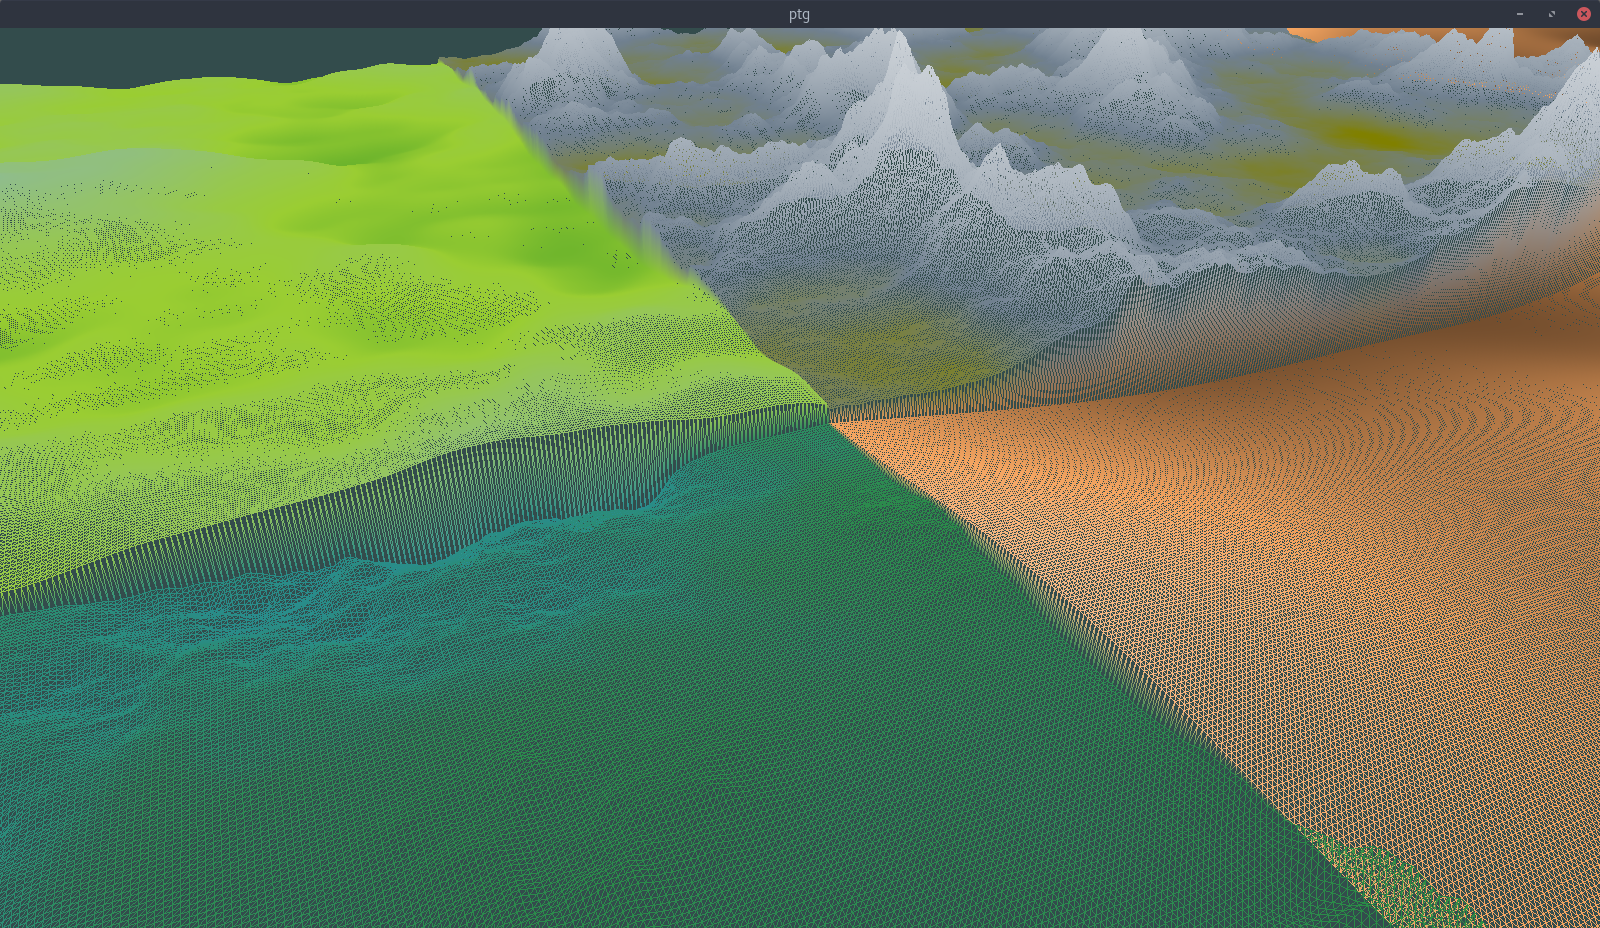
\includegraphics[width=.9\textwidth]{img/border/a9/1s.png}
        \caption{Ângulo 1 sem interpolação.}
        \label{fig:img_border_a9_1s}
    \end{figure}
    
\end{frame}


\begin{frame}{Fronteiras}
    \begin{figure}[H]
        \centering
        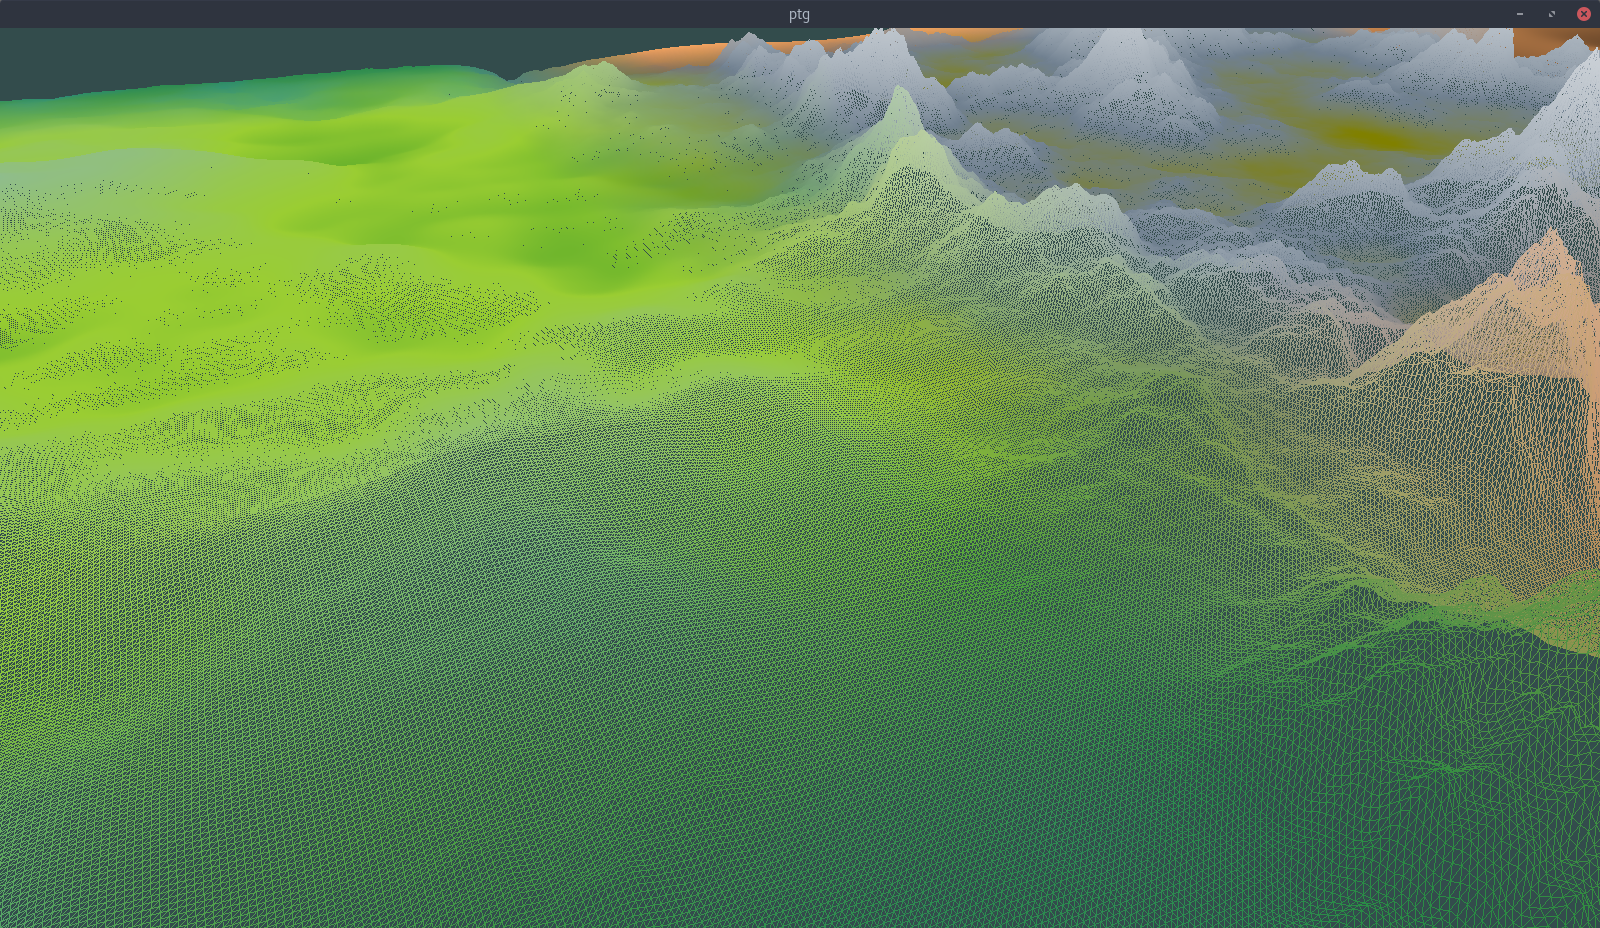
\includegraphics[width=.9\textwidth]{img/border/a9/1c.png}
        \caption{Ângulo 1 com interpolação.}
        \label{fig:img_border_a9_1c}
    \end{figure}
    
\end{frame}

\begin{frame}{Fronteiras}
    \begin{figure}[H]
        \centering
        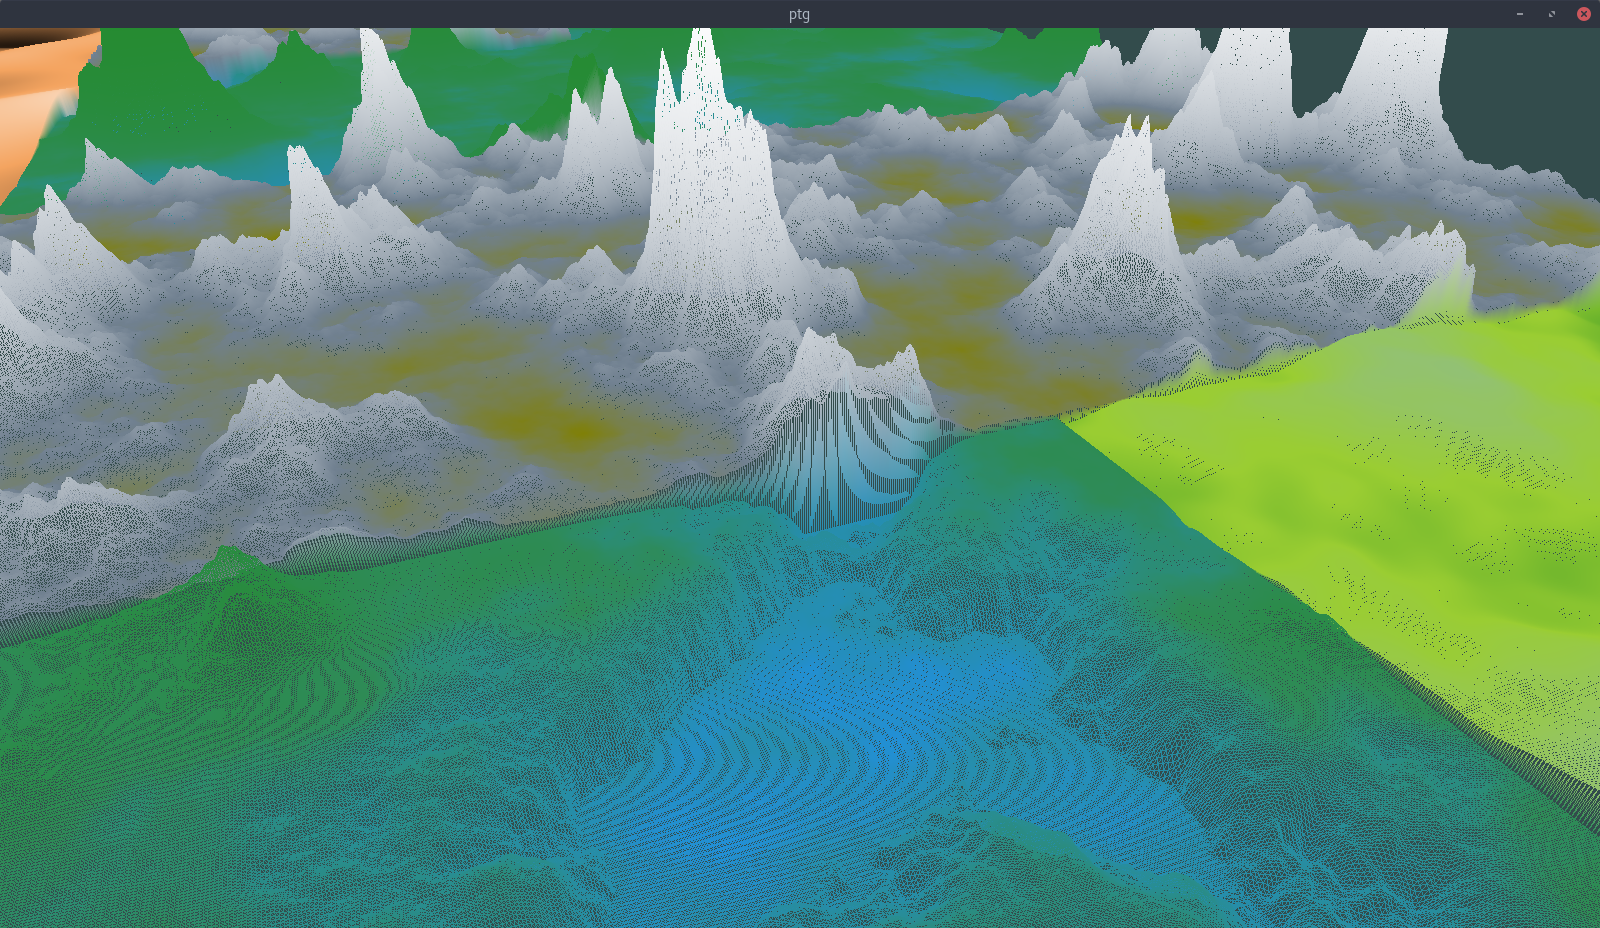
\includegraphics[width=.9\textwidth]{img/border/a9/2s.png}
        \caption{Ângulo 2 sem interpolação.}
        \label{fig:img_border_a9_2s}
    \end{figure}
    
\end{frame}


\begin{frame}{Fronteiras}
    \begin{figure}[H]
        \centering
        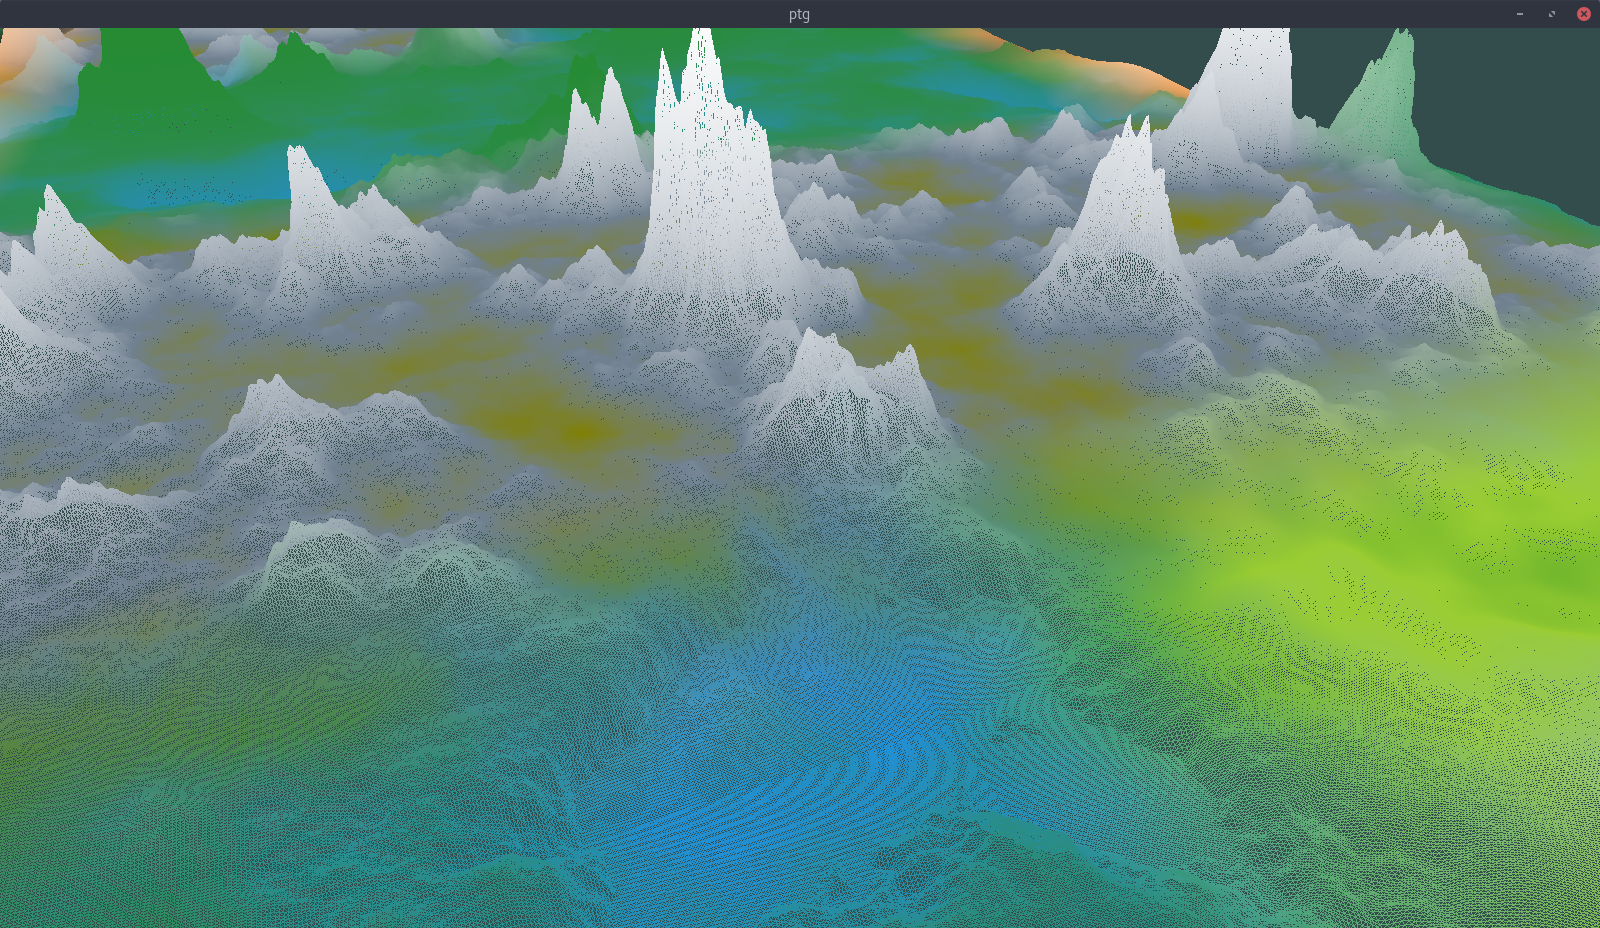
\includegraphics[width=.9\textwidth]{img/border/a9/2c.png}
        \caption{Ângulo 2 com interpolação.}
        \label{fig:img_border_a9_2c}
    \end{figure}
    
\end{frame}

\begin{frame}{Fronteiras}
    \begin{figure}[H]
        \centering
        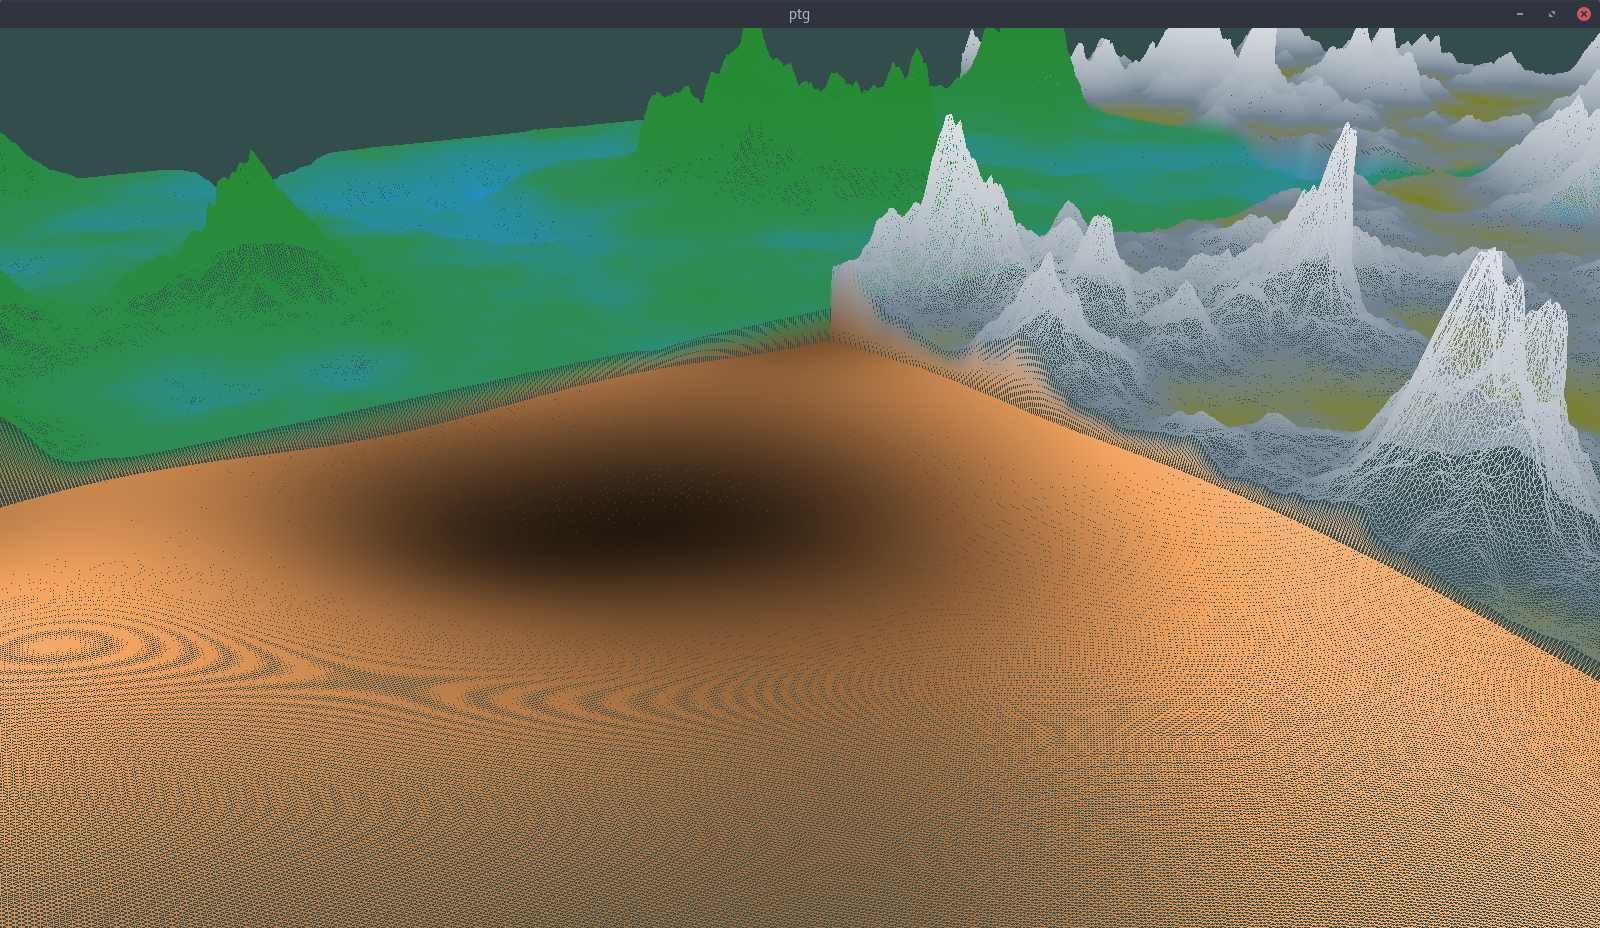
\includegraphics[width=.9\textwidth]{img/border/a9/3s.png}
        \caption{Ângulo 3 sem interpolação.}
        \label{fig:img_border_a9_3s}
    \end{figure}
    
\end{frame}


\begin{frame}{Fronteiras}
    \begin{figure}[H]
        \centering
        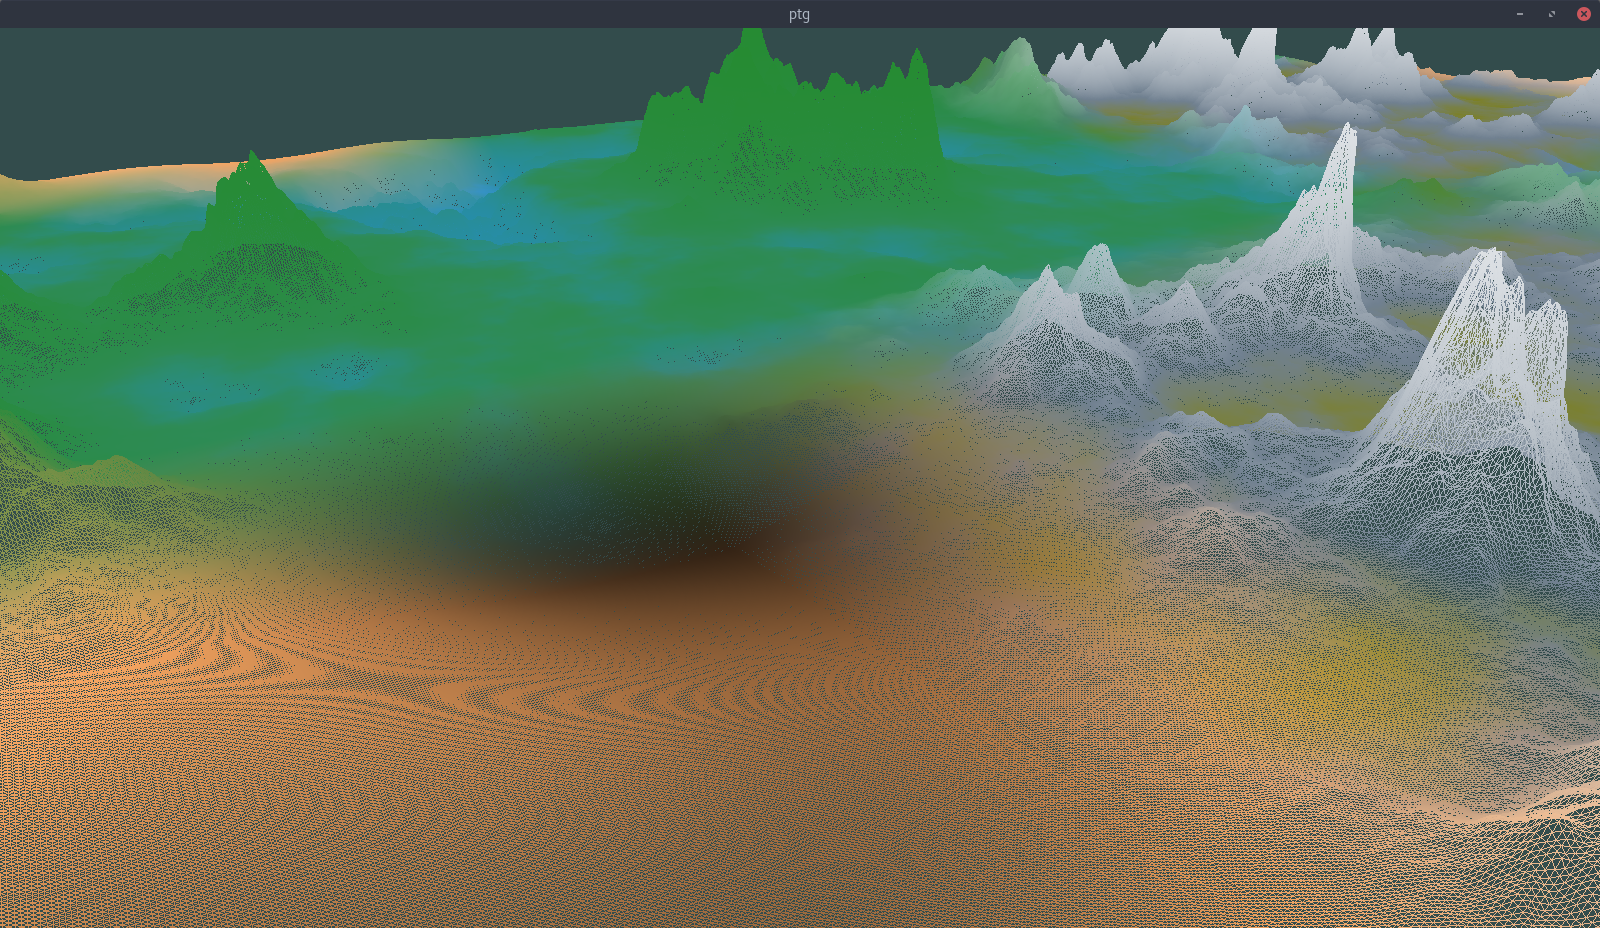
\includegraphics[width=.9\textwidth]{img/border/a9/3c.png}
        \caption{Ângulo 3 com interpolação.}
        \label{fig:img_border_a9_3c}
    \end{figure}
    
\end{frame}

\begin{frame}{Fronteiras}
    \begin{figure}[H]
        \centering
        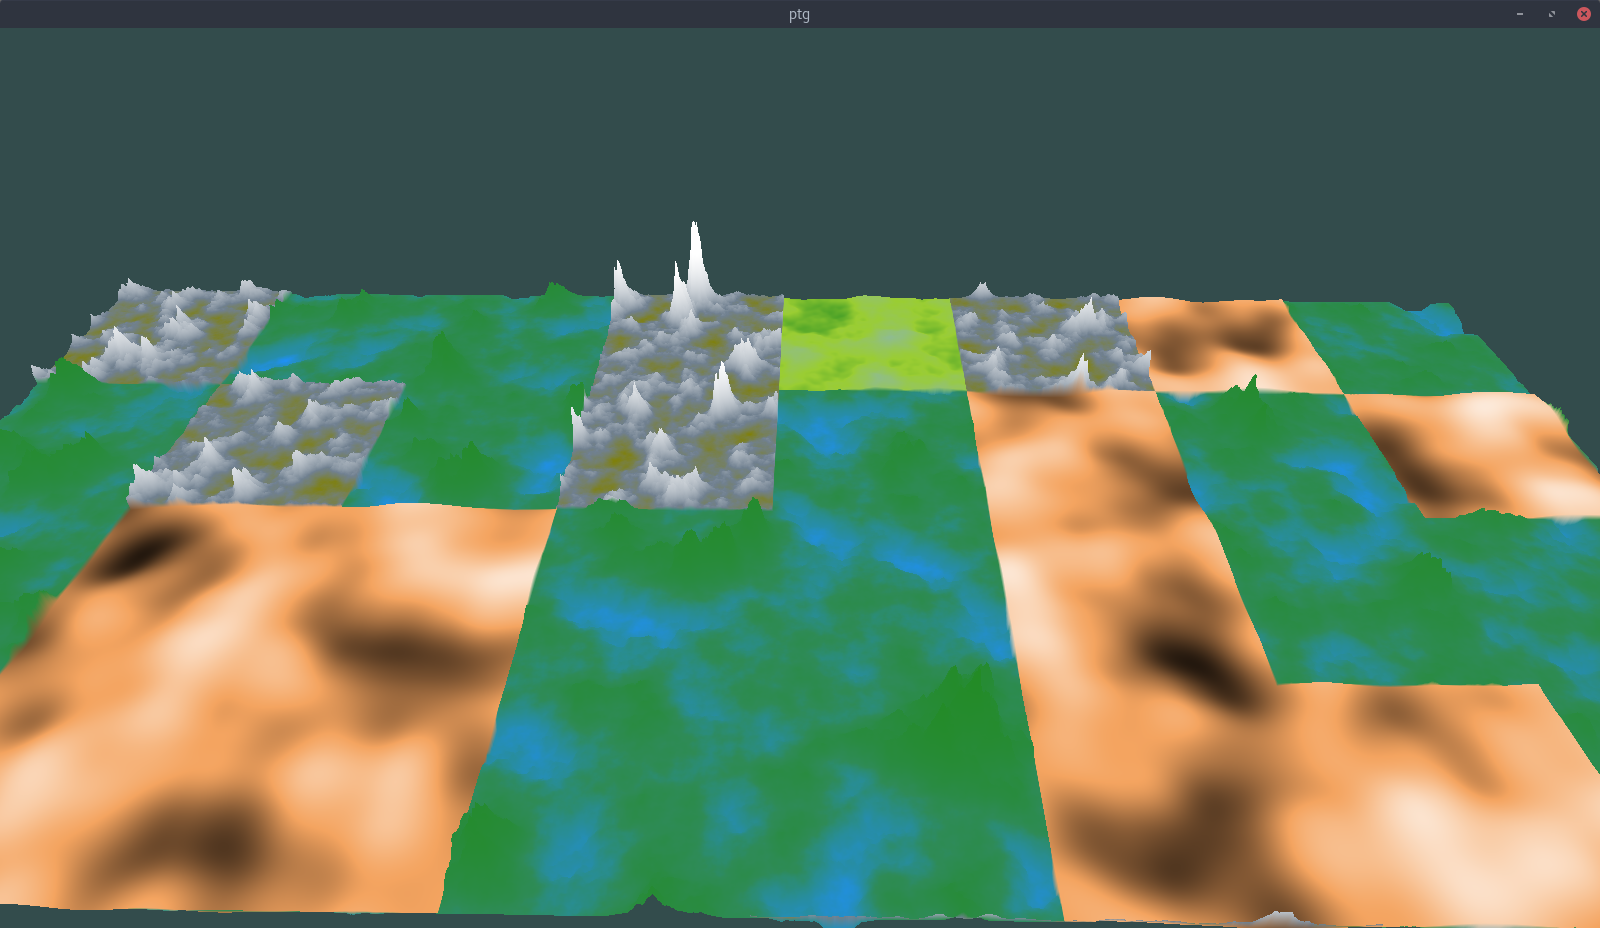
\includegraphics[width=.9\textwidth]{img/border/a9/4s.png}
        \caption{Ângulo 4 sem interpolação.}
        \label{fig:img_border_a9_4s}
    \end{figure}
    
\end{frame}


\begin{frame}{Fronteiras}
    \begin{figure}[H]
        \centering
        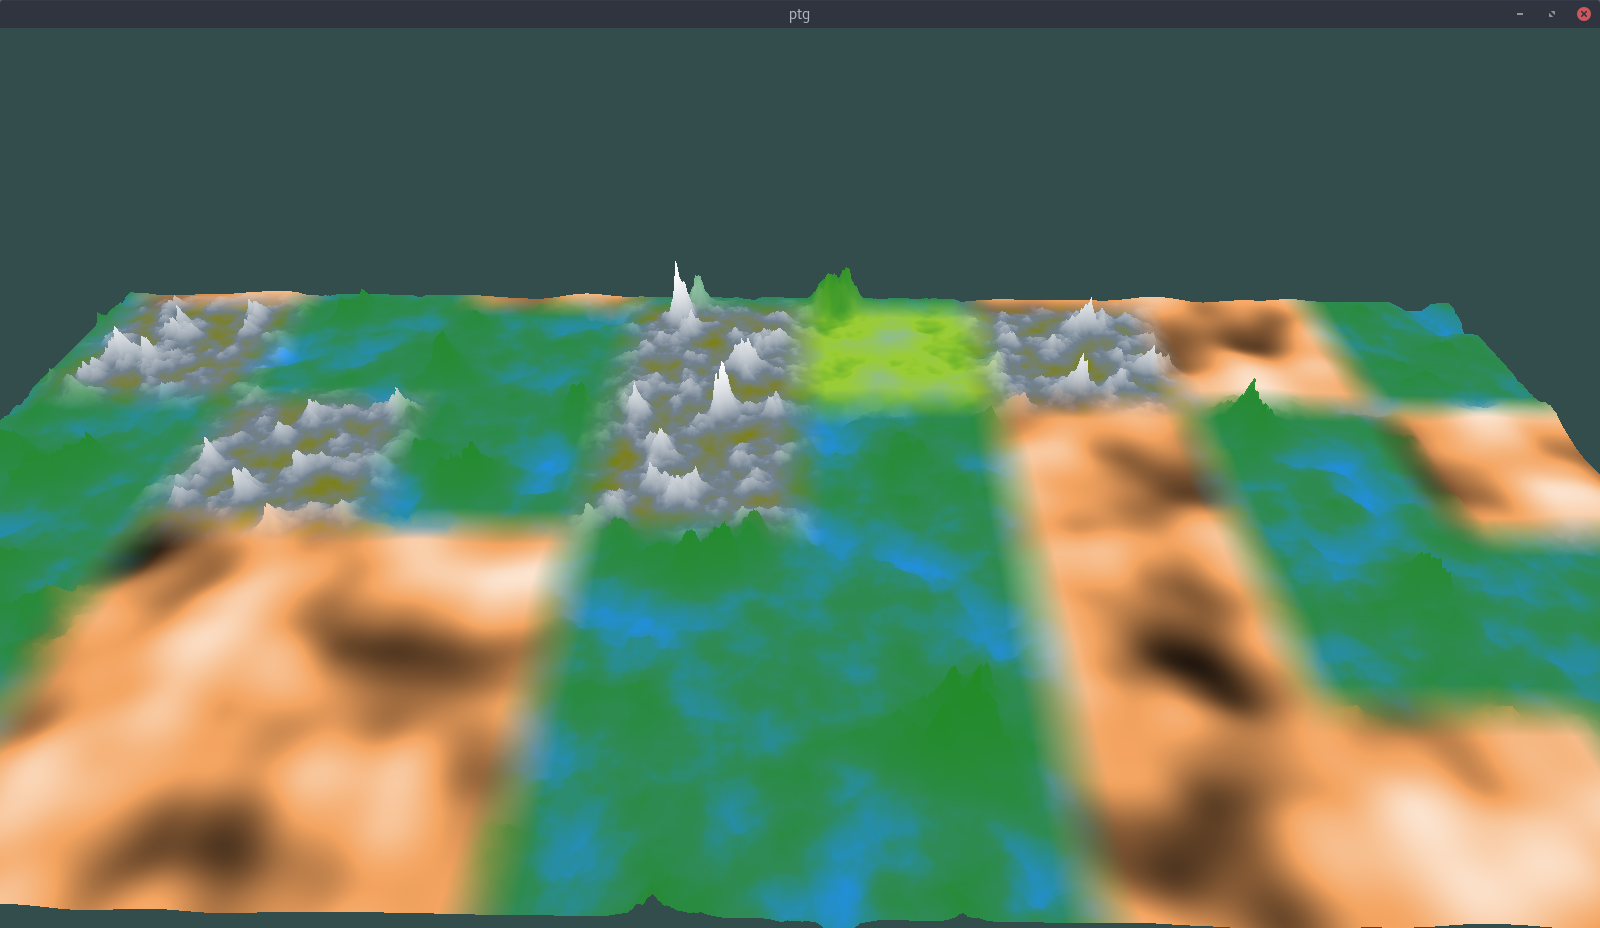
\includegraphics[width=.9\textwidth]{img/border/a9/4c.png}
        \caption{Ângulo 4 com interpolação.}
        \label{fig:img_border_a9_4c}
    \end{figure}
    
\end{frame}

\begin{frame}{Fronteiras}
    \begin{itemize} \setlength\itemsep{1em}
        \item Com diferentes parâmetros de $l$.
    \end{itemize}
    
    
\end{frame}

\begin{frame}{Fronteiras}
    \begin{figure}[H]
        \centering
        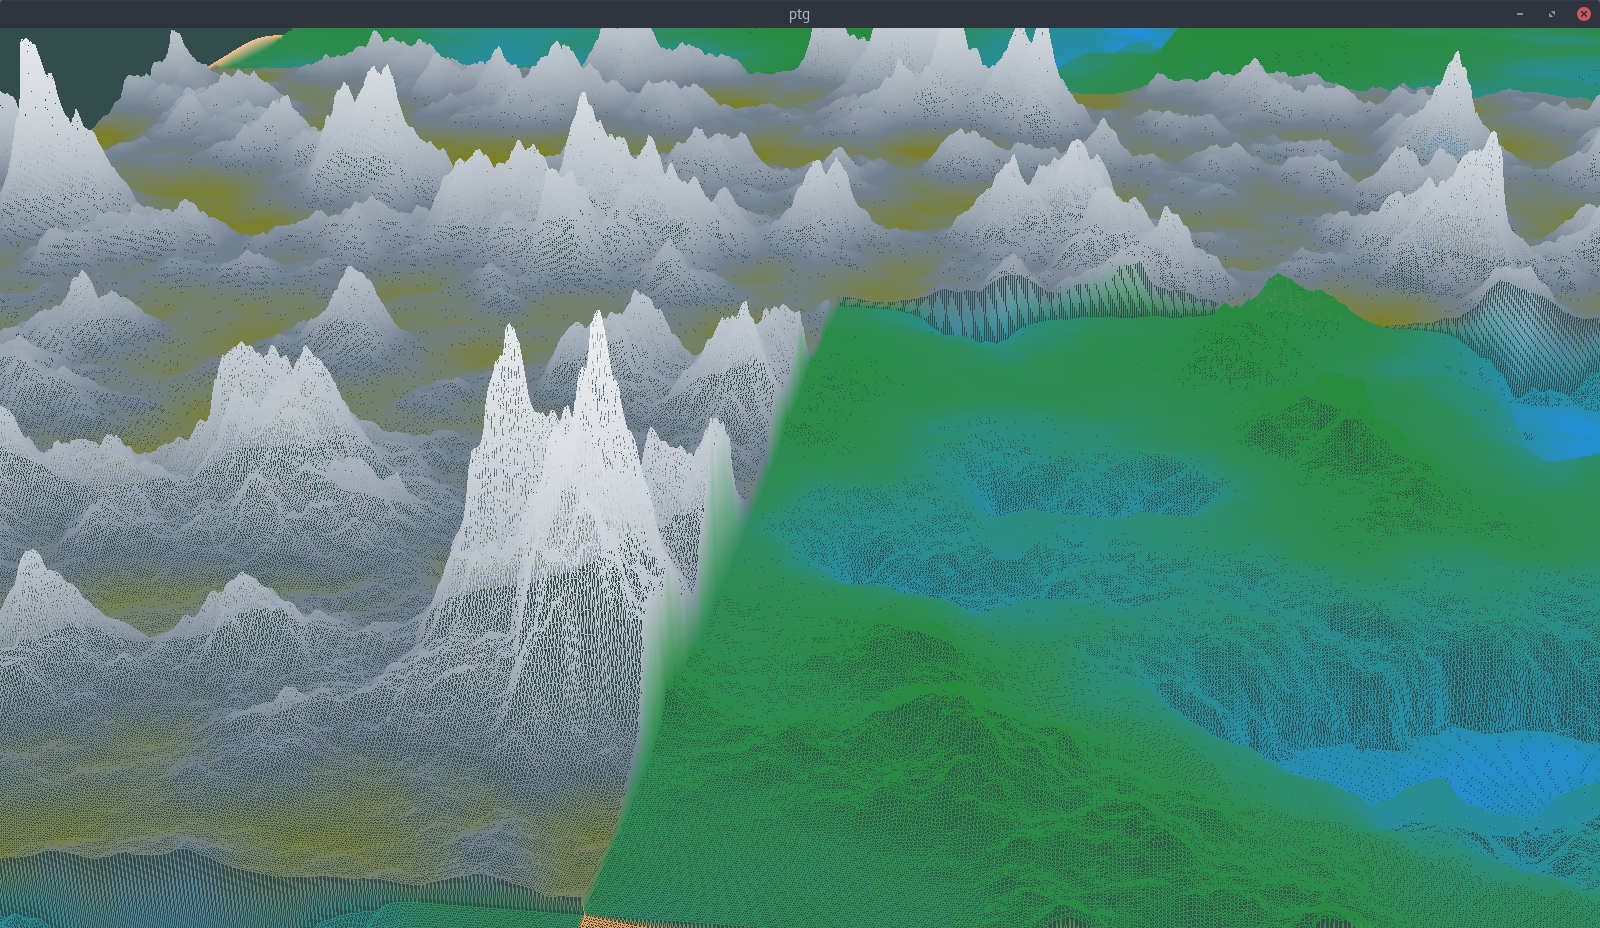
\includegraphics[width=.9\textwidth]{img/borders/0lm.png}
        \caption{Sem interpolação.}
        \label{fig:img_borders_0lm}
    \end{figure}
    
\end{frame}

\begin{frame}{Fronteiras}
    \begin{figure}[H]
        \centering
        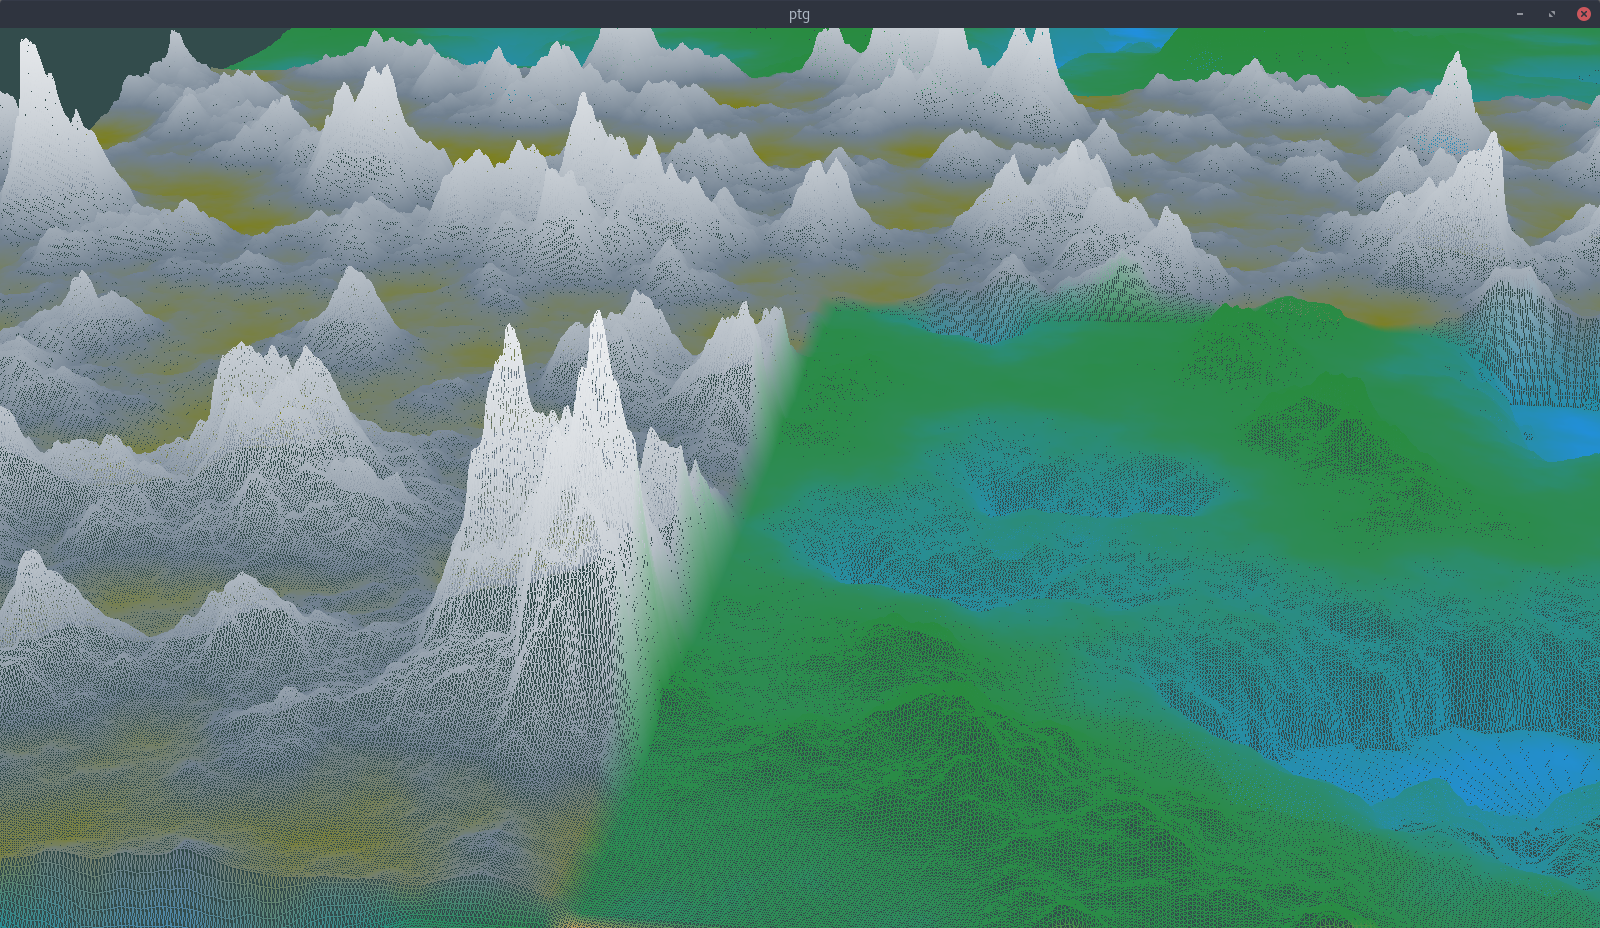
\includegraphics[width=.9\textwidth]{img/borders/8lm.png}
        \caption{interpolação com $l = 8$.}
        \label{fig:img_borders_8lm}
    \end{figure}
    
\end{frame}

\begin{frame}{Fronteiras}
    \begin{figure}[H]
        \centering
        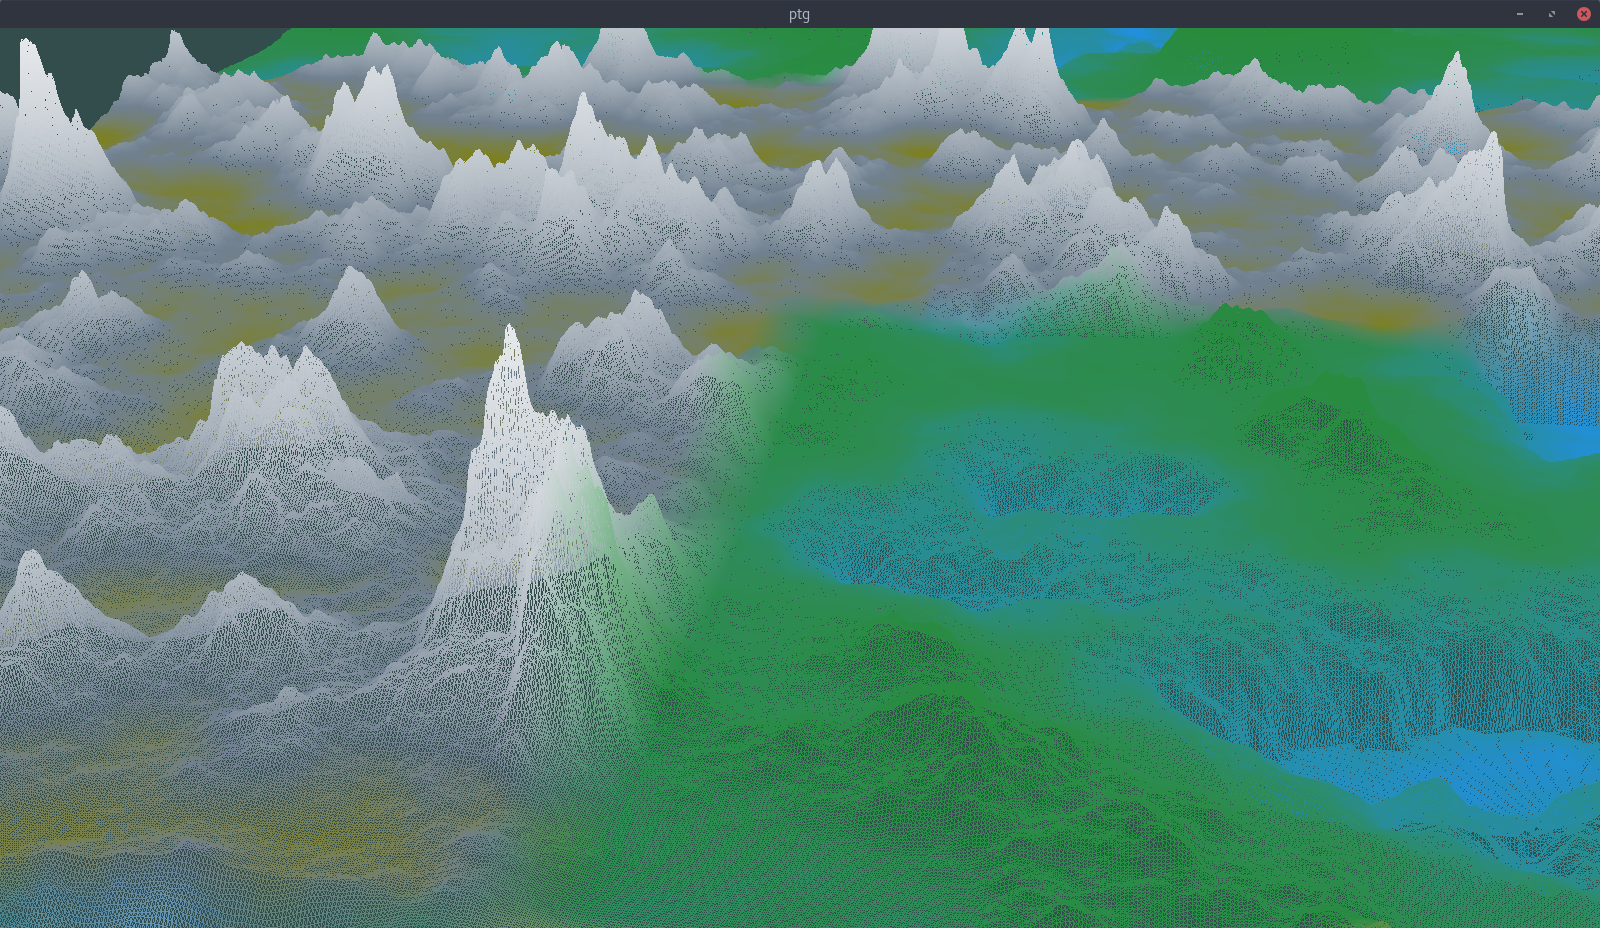
\includegraphics[width=.9\textwidth]{img/borders/32lm.png}
        \caption{interpolação com $l = 32$.}
        \label{fig:img_borders_32lm}
    \end{figure}
    
\end{frame}

\begin{frame}{Fronteiras}
    \begin{figure}[H]
        \centering
        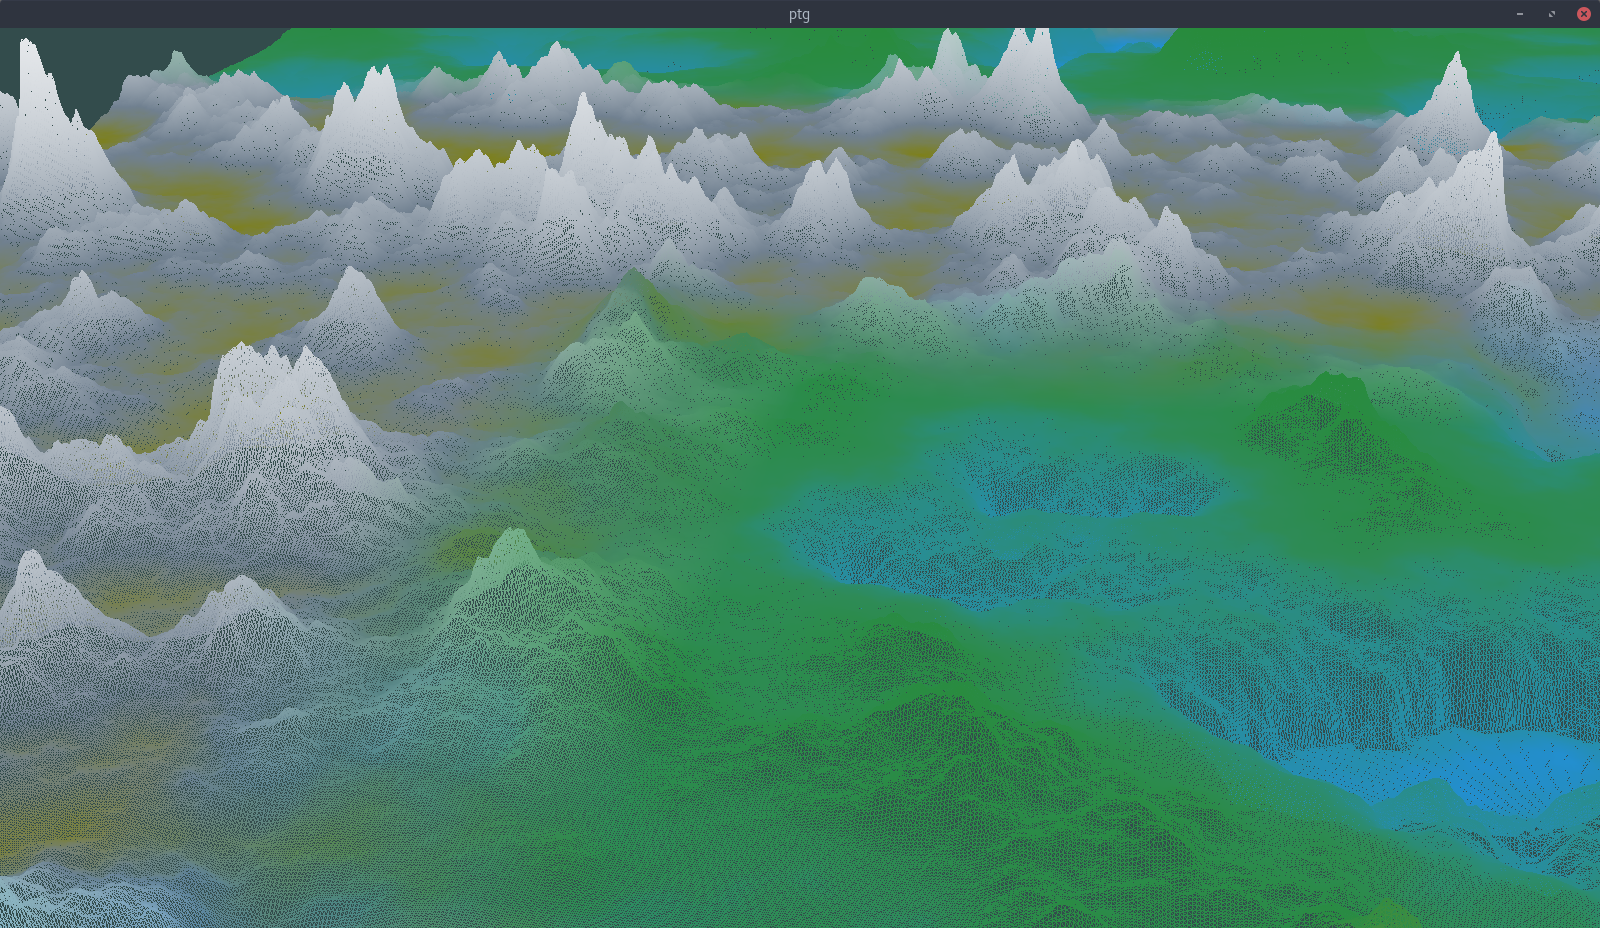
\includegraphics[width=.9\textwidth]{img/borders/128lm.png}
        \caption{interpolação com $l = 128$.}
        \label{fig:img_borders_128lm}
    \end{figure}
    
\end{frame}

\begin{frame}{Fronteiras}
    \begin{figure}[H]
        \centering
        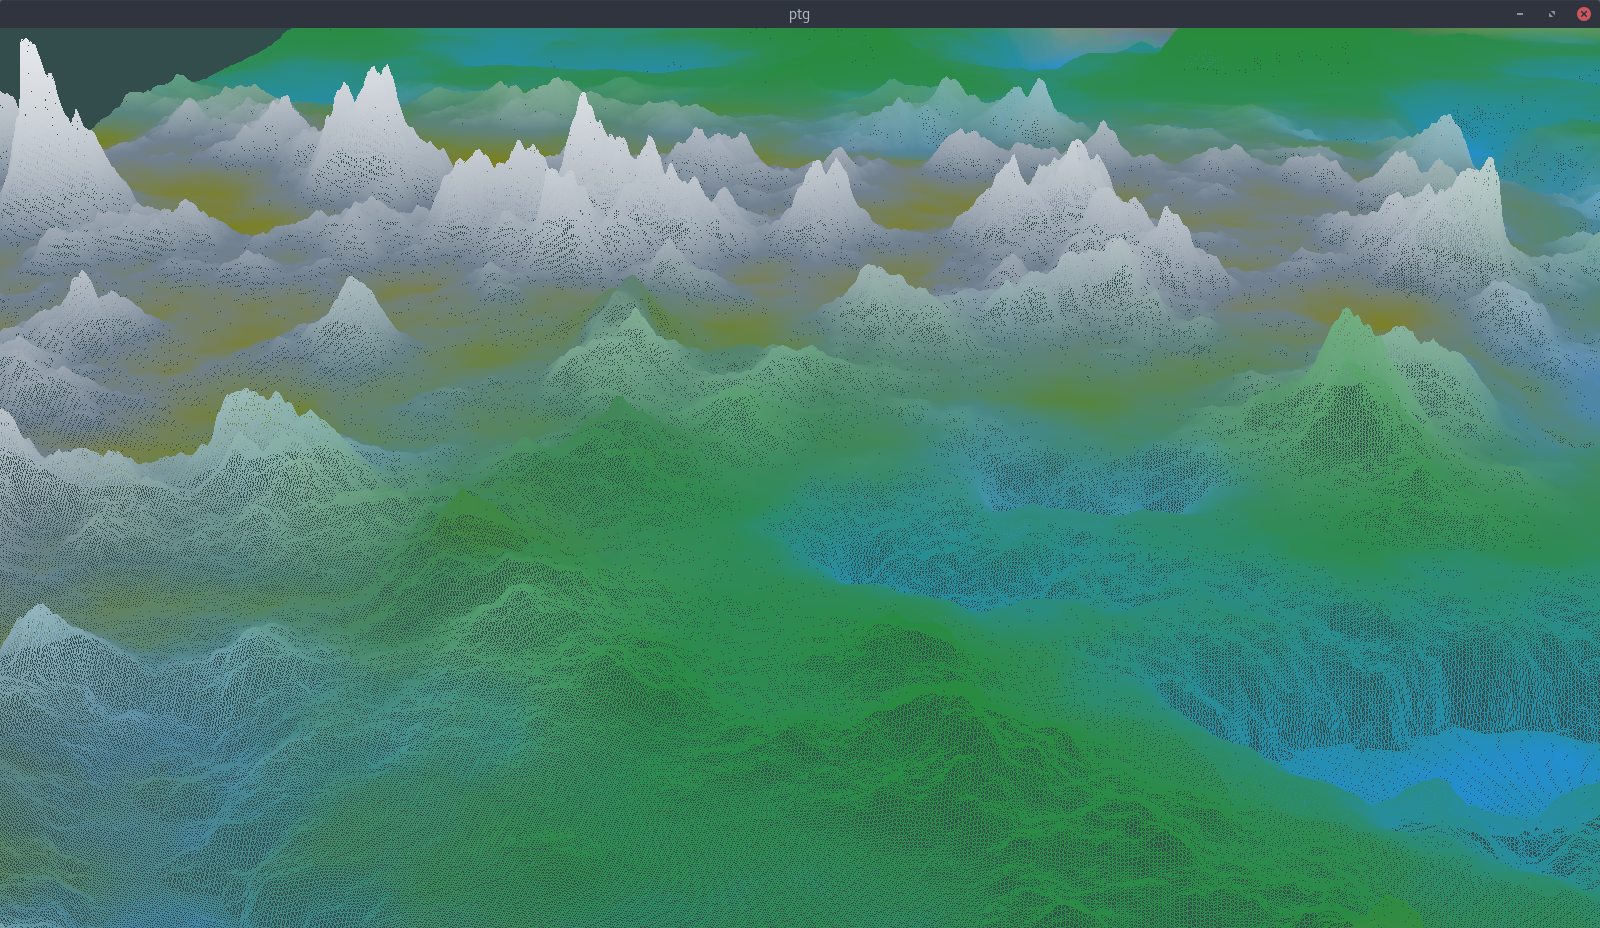
\includegraphics[width=.9\textwidth]{img/borders/255lm.png}
        \caption{interpolação com $l = 255$.}
        \label{fig:img_borders_255lm}
    \end{figure}
    
\end{frame}